\documentclass[a4paper,14pt]{article}

\usepackage{comment} % Para comentar várias linhas ao mesmo tempo

%matemática
\usepackage{amsmath}
\usepackage{amssymb}

%diagramação
\usepackage{extsizes}
\everymath{\displaystyle}
\usepackage{geometry}
\usepackage{fancyhdr}
\usepackage{multicol}
\usepackage{graphicx}
\usepackage[brazil]{babel}
\usepackage[shortlabels]{enumitem}
\usepackage{cancel}
\usepackage{textcomp}
\usepackage{tcolorbox}

%tabelas
\usepackage{array} % Para melhor formatação de tabelas
\usepackage{longtable}
\usepackage{booktabs}  % Para linhas horizontais mais bonitas
\usepackage{float}   % Para usar o modificador [H]
\usepackage{caption} % Para usar legendas em tabelas
\usepackage{wrapfig} % Para usar tabelas e figuras flutuantes


%tikzpicture
\usepackage{tikz}
\usepackage{scalerel}
\usepackage{pict2e}
\usepackage{tkz-euclide}
\usetikzlibrary{calc}
\usetikzlibrary{patterns,arrows.meta}
\usetikzlibrary{shadows}
\usetikzlibrary{external}


%pgfplots
\usepackage{pgfplots}
\pgfplotsset{compat=newest}
\usepgfplotslibrary{statistics}
\usepgfplotslibrary{fillbetween}

%colours
\usepackage{xcolor}



\columnsep=2cm
\hoffset=0cm
\textwidth=8cm
\setlength{\columnseprule}{.1pt}
\setlength{\columnsep}{2cm}
\renewcommand{\headrulewidth}{0pt}
\geometry{top=1in, bottom=1in, left=0.7in, right=0.5in}

\pagestyle{fancy}
\fancyhf{}
\fancyfoot[C]{\thepage}

\begin{document}
	
	\noindent\textbf{6FMA29 - Matemática} 
	
	\begin{center}O bloco retangular (Versão estudante)
	\end{center}
	
	\noindent\textbf{Nome:} \underline{\hspace{10cm}}
	\noindent\textbf{Data:} \underline{\hspace{4cm}}
	
	%\section*{Questões de Matemática}
	
	\begin{multicols}{2}
		\noindent O bloco retangular (ou paralelepípedo reto-retângulo) possui três dimensões (comprimento, largura e altura) e é formado por retângulos. Exemplos: tijolo, baú de um caminhão, caixa de sapatos, etc. \\
		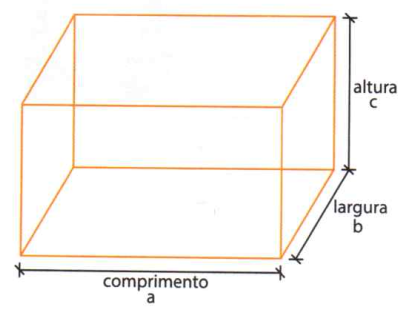
\includegraphics[width=1\linewidth]{6FMA29_imagens/imagem1} \\
		Os lados dos retângulos são chamados arestas. \\
		\noindent\textsubscript{-----------------------------------------------------------------------}
		\begin{enumerate} 
			\item Apresentamos abaixo figuras que representam objetos tridimensionais. Quais desses objetos têm a forma de blocos retangulares? Não se preocupe com detalhes, tais como cantos arredondados, frisos, orifícios, etc. O que interessa é a forma aproximada. \\
			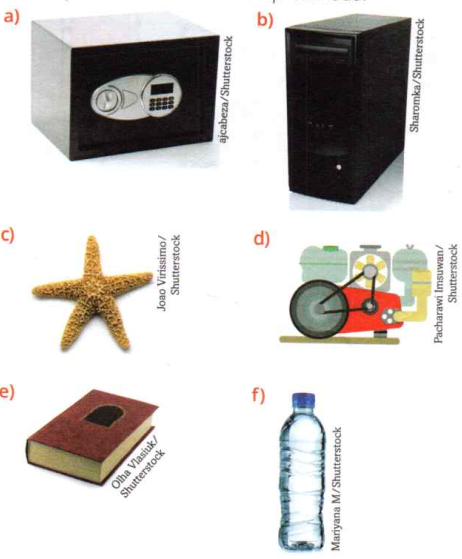
\includegraphics[width=1\linewidth]{6FMA29_imagens/imagem2} \\\\\\\\\\\\\\\\\\
			\item No máximo, quantas faces de uma caixa de sapatos você consegue enxergar? \\\\\\\\\\\\\\\\
			\item Quantas arestas de medidas diferentes um bloco retangular pode ter no máximo? \\\\\\\\\\\\\\\\\\
			\item O que você pode afirmar a respeito das faces opostas de um bloco retangular? \\\\\\\\\\\\\\\\\\
			\item Para montar um bloco retangular de arame com 45 cm de comprimento, 30 cm de largura e 12 cm de altura, que quantidade de arame iremos usar? \\\\\\\\\\\\\\\\\\\\
			%102 a 106
			\item Que quantidade de arame é usada para montar um bloco retangular de dimensões 32 $\times$ 16 $\times$ 20 cm? \\\\\\\\\\\\\\\\\\\\\\\\\\
			\item Uma formiga faminta estava num dos vértices de um bloco retangular feito apenas com varetas, quando percebeu que havia uma migalha de pão no vértice do bloco mais distante possível. Sabendo que o bloco tem dimensões 5 $\times$ 12 $\times$ 13 m, calcule a distância mínima que a formiga deverá percorrer para saciar seu apetite. \\\\\\\\\\\\\\\\\\\\\\\\
			\item Uma baratinha encontra-se num dos vértices de um bloco retangular feito apenas com varetas e percebeu que há uma migalha de doce no vértice do outro lado do bloco, justamente naquele mais distante possível. O bloco tem dimensões 26 $\times$ 20 $\times$ 18 cm. Quanto a baratinha vai ter que andar, no mínimo, para chegar ao seu petisco? \\\\\\\\\\\\\\\\\\\\\\\\\\
			\item Com 64 cubos iguais pode-se construir um cubo maior. Qual é a medida da aresta do cubo maior, em centímetros, se os cubos menores têm aresta de 20 mm? \\\\\\\\\\\\\\\\\\\\
			\item Identifique as medidas representadas pelas letras, $x$, $y$ e $z$ indicadas nas figuras a seguir, formadas pela junção de paralelepípedos retos. \\
			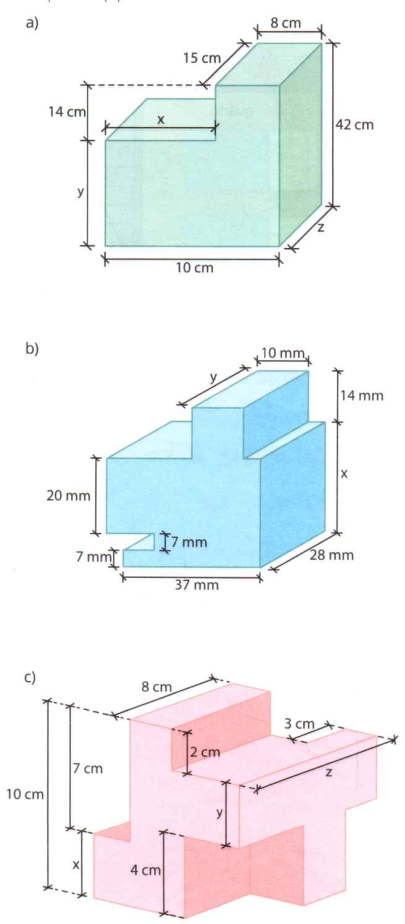
\includegraphics[width=1\linewidth]{6FMA29_imagens/imagem3} \\
			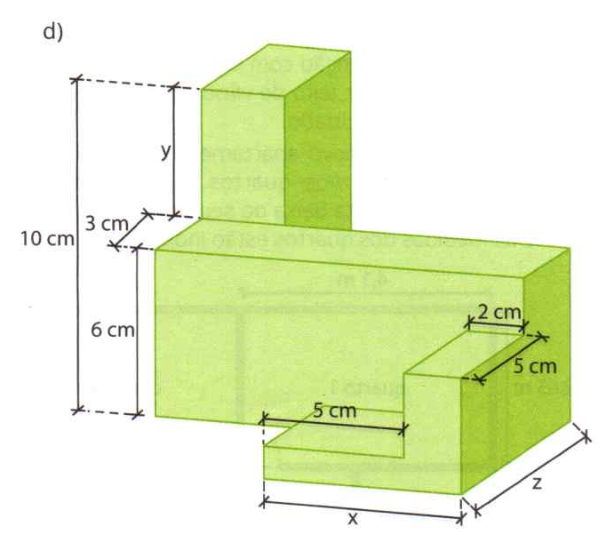
\includegraphics[width=0.8\linewidth]{6FMA29_imagens/imagem4}
		\end{enumerate}
	\end{multicols}
\end{document}